\section{Aufbau}
\label{sec:Aufbau}
Zur Durchführung der Messungen wird ein Ultraschallgenerator mit einer passenden Ultraschallsonde mit einer Frequenz von $\SI{2}{\mega\hertz}$ benutzt. Der Ultraschallgenerator besitzt zudem einen Regler DEPTH und SAMPLE VOLUME. Zur Auswertung der Messwerte wird ein Computer mit der Software FlowView verwendet. Die Flüssigkeit aus Wasser, Glycerin und Glaskugeln wird von einer Zentrifugalpumpe durch drei Rohre mit verschiedenen Innen- und Außendurchmessern gepumpt. Der Durchfluss an der Pumpe kann von $\SI{0}{\liter\per\minute}$ bis $\SI{10}{\liter\per\minute}$ variiert werden. Um reproduzierbare Winkel zwischen der durchschnittlichen Strömungsrichtung und der Ultraschallsonde zu gewährleisten werden Doppler-Prismen mit drei verschiedenen festen Winkeln $\theta$ verwendet. Es gibt jeweils ein Prisma für jedes Rohr, welches in Abbildung \ref{fig:prisma} dargestellt ist. Es gilt nach dem Brechungsgesetz für die Dopplerwinkel 
\begin{equation}
	\alpha = \SI{90}{\degree} - \arcsin\left(\sin(\theta) \frac{c_\text{L}}{c_\text{P}}\right)\text{.}
\end{equation}
Hierin ist $c_\text{L}$ die Schallgeschwindigkeit in der Flüssigkeit und $c_\text{P}$ die Schallgeschwindigkeit in dem Prisma.
\begin{figure}
	\centering
	\caption{Darstellung eines in dem Versuch verwendeten Prismas \cite{US3}.}
	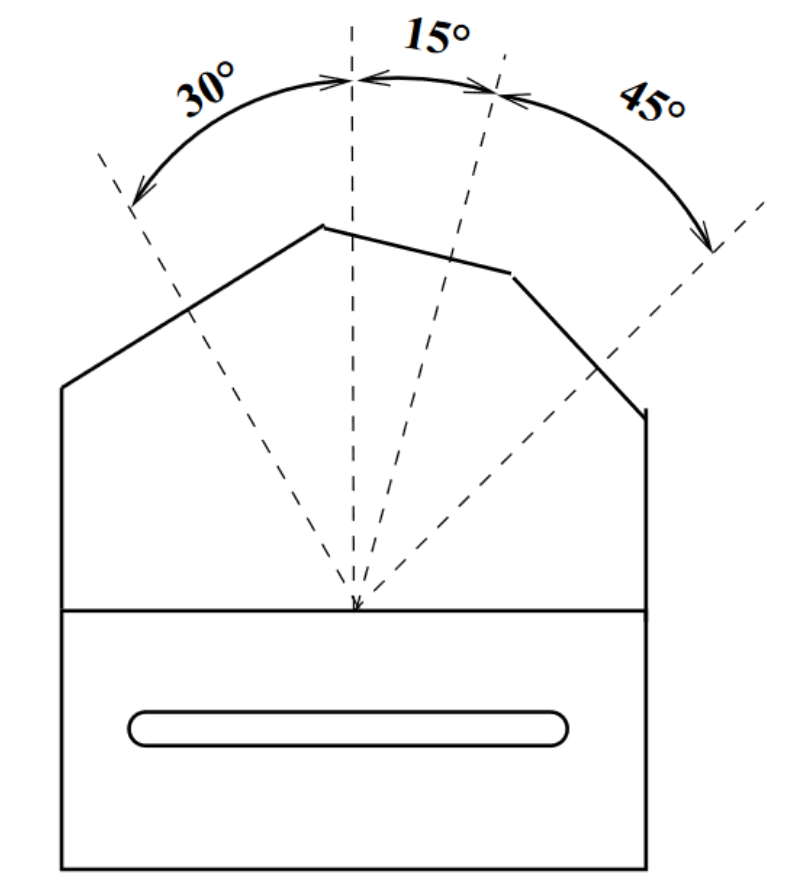
\includegraphics[width=\linewidth-70pt,height=0.3\textheight,keepaspectratio]{content/images/prisma.png}
	\label{fig:prisma}
\end{figure}